\chapter{Implementation}
\label{chap:impl}

In the previous chapter the conceptual approach to the realisation of the PSS-IF \gls{poc} was described. In particular, the latter sections of \chapref{chap:approach} describe the principles behind the chosen transformation method. In this context, this chapter focuses on the implementation of the framework. The chapter is structured as follows: \secref{sec:impl:technology} describes the technology stack used for the implementation. In \secref{sec:impl:principles} the adopted software development guiding principles are presented. Thereafter, \secref{sec:impl:structure} provides an overview of the project structure. \secref{sec:impl:components} follows with a description of each component of the PSS-IF \gls{poc} and, finally, \secref{sec:impl:process} describes the import and export processes and the collaboration of all components of the framework.

\section{Technology Stack}
\label{sec:impl:technology}

This section defines the technologies used for the implementation of the PSS-IF \gls{poc}. Each of the following subsections addresses a particular aspect of the technological stack. Note that all the software and tools used for the realization of the \gls{poc} are widely accepted industry standards.

\subsection{Programming Language}

To enable an easier and more rapid development of the prototype, a high-level programming language can better be utilized. Due to previous experience and know-how, the authors have chosen the Java Programming Language \cite{ref:java}. Furthermore, the code is compliant with Java version 7, as distributed by Oracle. 

\subsection{Source Code Management}

For improved parallelisation, better code maintenance and easier documentation, a distributed version control system can be used. While there are numerous alternatives, the authors have chosen git \cite{ref:git} as a modern and powerful solution.

\subsection{Build Process and Dependency Management}

For the automated build process, as well as for the management of dependencies to external libraries, Apache Maven\cite{ref:maven} has been used.

\subsection{Test Framework}

For the execution of automated tests, JUnit\cite{ref:junit}, an industry standard framework within the Java universe, has been used.

\subsection{Used Libraries}

Next to the libraries provided by Oracle's Standard Java Runtime Environment, the following additional libraries have been used:

\paragraph{apache-compress \cite{ref:compress}} An \gls{api} for the manipulation of different kinds of compressed files. In the scope of the \gls{poc}, the \gls{api} is used in the Visio \cite{ref:visio} processing component, for the zipping and unzipping of Visio files.

\paragraph{guava \cite{ref:guava}} Google Guava is a set of common libraries, mainly developed by Google. The package includes useful \glspl{api} for the manipulation of collections, the usage of functions and predicates, and others.

\paragraph{emf \cite{ref:emf}} The \gls{emf} library is used for the serialization and de-serialization of eCore \cite{ref:emf} and \gls{xmi} \cite{ref:xmi} files, enabling the processing of SysML4Mechatronics data.

\paragraph{junit} JUnit is an industry standard unit-testing framework.

\section{Guiding Principles}
\label{sec:impl:principles}

During the design and implementation of the PSS-IF \gls{poc} the authors have followed the principles and best-practices for software development. Some of the guiding principles were the following:

\paragraph{Standardization:} Usage of widely used and accepted industry-standard tools, technologies and formats, to render the produced solution more accessible to new developers and compliant to other pieces of software.

\paragraph{Patterns:} To maximize code quality and understandability, common architecture and design patterns have been utilized.

\paragraph{Object-Orientation:} The code is developed in accordance with the paradigms of the Java programming language -- it is mostly object-oriented and imperative.

\paragraph{Separation of Concerns:} The implementation follows the separation of concerns paradigm.

\section{Project Structure}
\label{sec:impl:structure}

The PSS-IF \gls{poc} is developed as an Apache maven project, further divided into a root project, called ''\textbf{pssif}'' and a number of sub-modules. The root project is used for the provision of common development and  build configuration, as for example the specification of common dependencies with a fixed version over all modules. This avoids redundancy and improves the manageability of the developed code. Each of the modules represents a component of the PSS-IF \gls{poc} architecture on a coarse level of abstraction. While it is possible to establish a project with fine-grained maven modularity, division in fine-grained modules would make it more difficult to capture the project structure. This is why the authors have tried to find a balance between capturing coarse-level architectural concepts through maven modularization and fine-grained modularization of components, which is achieved through the packaging mechanism of the Java programming language.

This section covers the coarse-grained separation realized through maven modularization, while \secref{sec:impl:components} is concerned with the fine-grained architectural modularization of the project. Currently, the PSS-IF \gls{poc} consists of three modules, as depicted in  \figref{fig:structure}.

\begin{figure}
\centering
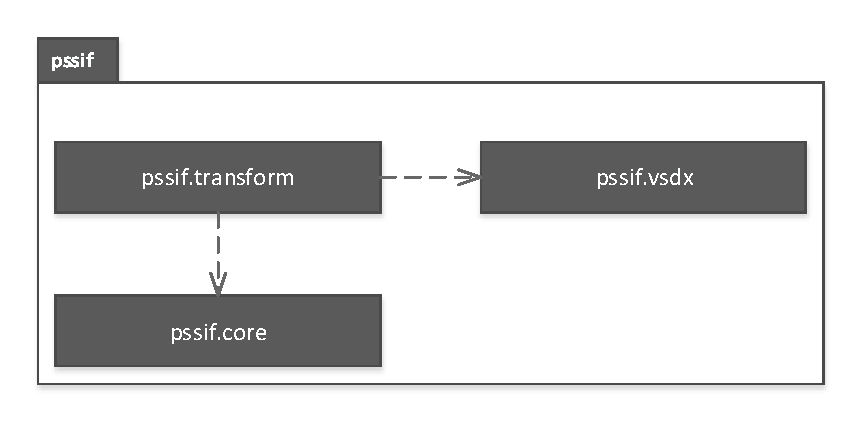
\includegraphics[width=0.8\textwidth]{figures/project-structure.pdf}
\caption{Project Structure}
\label{fig:structure}
\end{figure}

\paragraph{Core} The ''\textbf{core}'' maven module contains the fundamental \gls{api} of the framework. This \gls{api} defines the concepts through which the PSS-IF \gls{dsl} is described, such as Metamodel, Model, NodeTypes, Nodes etc. Furthermore, the core module provides an implementation layer for the concepts of the PSS-IF \gls{dsl}, as well as a number of common utilities, like for example a generator for the canonic PSS-IF Metamodel, as depicted in \figref{fig:canonic}.

\paragraph{Transform} The ''\textbf{transformation}'' maven module provides the \gls{api} used for the definition and execution of transformations, as well as for input and output (I/O) operations. Next to the \glspl{api}, this module also contains their implementation, as well as a number of commonly used helping utilities, concerned with transformation or the serialization to or de-serialization from external formats. Finally, this module contains implementations for the supported source and target languages.

\paragraph{VSDX} The ''\textbf{vsdx}'' module is a dedicated module which provides an API and an implementation for the processing of Microsoft Visio 2013 VSDX documents \cite{ref:visio}. The module defines an abstraction layer describing the structure of a Visio document in an object-oriented fashion, and is used for the serialization and de-serialization of VSDX files.

\section{Components}
\label{sec:impl:components}

After, in the previous section, the coarse-level division of the PSS-IF \gls{poc} parts through maven modules was presented, this section focuses on a more detailed view on the architectural components of the tool. Each of the following subsections describes the function and structure of a specific component of the transformation framework \gls{poc}.

\subsection{Core}

The core is the central component of the framework and is responsible for the realization of key concepts, used for the definition and processing of transformations. The core encloses two major concepts -- those of a \texttt{Metamodel} and a \texttt{Model}, which were already presented in \chapref{chap:approach}.

\subsubsection{Metamodel}

\begin{figure}
\centering
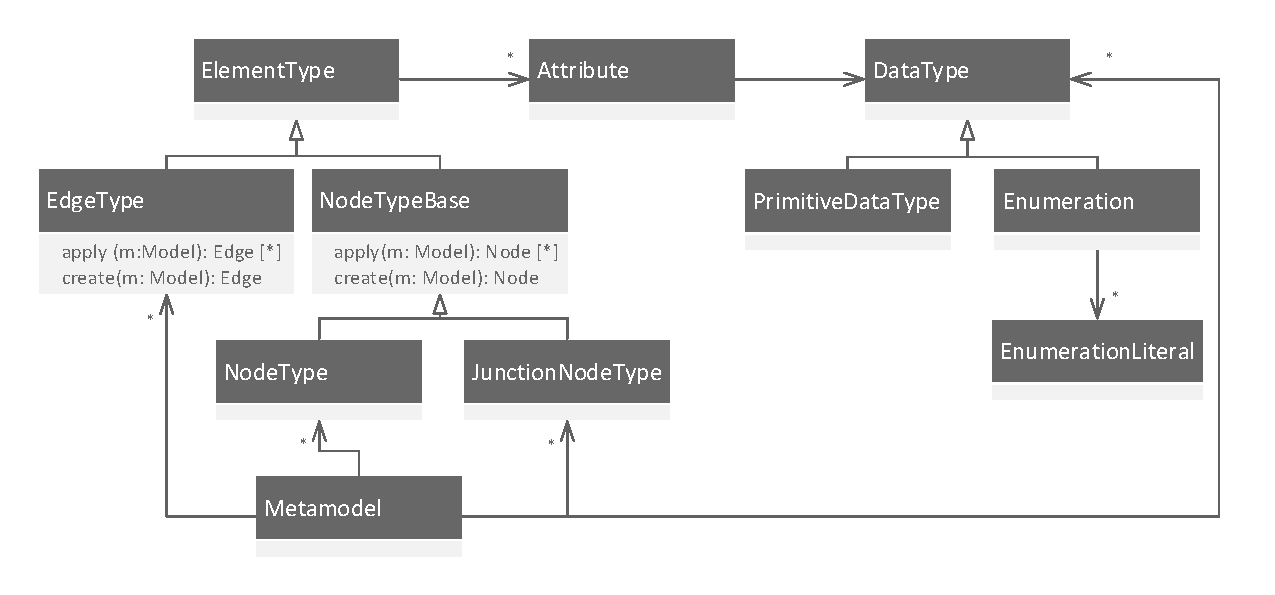
\includegraphics[width=\textwidth]{figures/metamodel.pdf}
\caption{Metamodel API}
\label{fig:metamodel}
\end{figure}

The \texttt{Metamodel} (see \figref{fig:metamodel}) is a concept which enables the users of the framework to define the structure of their data. In this sense, a \texttt{Metamodel} also defines, on the abstract syntax level, the language in which the elements of a PSS-IF \texttt{Model} are described. A parallel in the domain of the \gls{xml} is the \gls{xsd} \cite{ref:xsd}. In essence, a PSS-IF \texttt{Metamodel} is the schema definition in accordance to which a particular \texttt{Model} is created and processed.

A PSS-IF \texttt{Metamodel} captures a number of concepts. In particular, it consists of \texttt{NodeType}s and \texttt{EdgeTypes}, i.e. elements which enable the user to define what kinds of nodes and edges their model may contain, what kinds of features they may have, and how they may relate to each other. Furthermore, in the PSS-IF \gls{poc}, inheritance relations can be defined between both \texttt{NodeType} and \texttt{EdgeType}.

\paragraph{Node Types}

\texttt{NodeType}s are used for the description of the different kinds of nodes in a model and have a number of features. All \texttt{NodeType}s are named and the name must be unique in the scope of all \texttt{NodeType}s and \texttt{EdgeTypes}s within a \texttt{Metamodel}. Furthermore, \texttt{NodeType}s can have a number of attributes, and are connected to other \texttt{NodeType}s over \texttt{EdgeType}s, which can be both incoming and outgoing.

There are two categories of \texttt{NodeType}s -- conventional ones and \texttt{JunctionNodeType}s. The latter actually describe nodes with edge semantics, i.e. they are used for the representation of hyper-edges.

\paragraph{Edge Types}

\texttt{EdgeType}s are used for the description of possible edges in a user's model. \texttt{EdgeType}s also have a name, which is unique in the scope of a \texttt{Metamodel}. For it to be possible to associate the same \texttt{EdgeType} with different pairs of \texttt{NodeType} instances, the concept of a \texttt{ConnectionMapping} is introduced. A \texttt{ConnectionMap\-ping} is an association assigned to a particular \texttt{EdgeType}, which includes an incoming and an outgoing \texttt{NodeType}.

To illustrate the usage of the \texttt{ConnectionMapping}, consider the following example: Assuming two \texttt{NodeType} instances, denoted ''State'' and ''Function'' and an \texttt{EdgeType} ''Control Flow'', which has to connect both node types in both directions. In the PSS-IF \gls{poc} this is achieved by instantiating a single \texttt{EdgeType} ''Control Flow'' and assigning two \texttt{ConnectionMapping} instances to it: one from ''State'' to ''Function'' and one from ''Function'' to ''State''.

\paragraph{Attributes}

For both \texttt{NodeType} and \texttt{EdgeType}, \texttt{Attribute}s can be defined. \texttt{At\-tribute}s are divided into \texttt{AttributeGroup}s, which can be used to separate different kinds of attributes conveniently, for example in a user interface. Furthermore, \texttt{Attribute}s are identified by their names, which have to be unique in the scope of the owning node or edge type. Also, each attribute has a \texttt{DataType}. The PSS-IF \gls{poc} defines a number of primitive data types, like \texttt{String}, \texttt{Integer}, \texttt{Date} and \texttt{Boolean}, and also provides the user with the ability to define custom enumeration data types. Finally, \texttt{Attribute} instances can optionally have a \texttt{Unit} associated with them, which can be particularly useful for numeric attributes. Finally, attributes are divided into categories. Currently, the following categories are defined: \texttt{Monetary}, \texttt{Weight}, \texttt{Density}, \texttt{Time}, \texttt{Geometry}, \texttt{MetaData} and \texttt{Material}.

\paragraph{Inheritance}

As already noted above, for both \texttt{NodeType} and \texttt{EdgeType}, inheritance relations can be defined. When a \texttt{NodeType} inherits from another \texttt{NodeType}, it holds that attribute groups and attributes are inherited from the parent.

\paragraph{Built-In Metamodel Elements}

Every PSS-IF Metamodel has a number of predefined elements. These are the root node and edge types. The root \texttt{NodeType} has the name ''\textbf{Node}'' and provides the following predefined Attributes:

\begin{itemize}
\item \textbf{id}: An identifier of data type \texttt{String} for the node instance of the node type, categorized as Metadata.
\item \textbf{name}: A name of data type \texttt{String}, categorized as \texttt{Metadata}.
\item \textbf{validity start}: A \texttt{Date}, designating the begin of the validity period of the given node, categorized as \texttt{Time}.
\item \textbf{validity end}: A \texttt{Date}, designating the end of the validity period of the given node, categorized as \texttt{Time}.
\item \textbf{version}: The version of the node, of data type \texttt{String}, categorized as \texttt{Metadata}.
\item \textbf{comment}: A comment of the node, of data type \texttt{String}, categorized as \texttt{Meta\-data}.
\end{itemize}

The root \texttt{EdgeType} '''\textbf{Edge}'' has all built-in attributes defined for the root \texttt{NodeType} ''Node'', and also an additional attribute \texttt{directed} of data type \texttt{Boolean} and categorized as \texttt{Metadata}. 

The root node and edge types are also the roots of the inheritance hierarchies for \texttt{NodeType} and \texttt{EdgeType} within a \texttt{Metamodel}. In this sense, any \texttt{NodeType} or \texttt{EdgeType} instance automatically inherits from the respective root type. Thus, it is guaranteed that the set of attributes provided above is automatically defined for all instances of both \texttt{NodeType} and \texttt{EdgeType}. If a node or edge type inherits from a non-root node or edge type, the attributes are inherited transitively, together with all attributes of all ancestors throughout the generalization closure.

\subsubsection{Model}

\begin{figure}
\centering
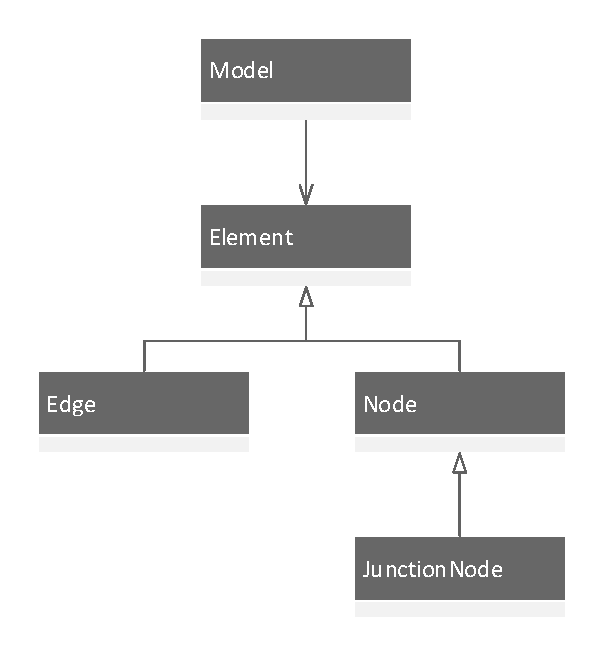
\includegraphics[scale=0.75]{figures/model.pdf}
\caption{Model API}
\label{fig:model}
\end{figure}

The second key component of the PSS-IF \gls{poc} core is the \texttt{Model} (see \figref{fig:model}), which can be seen as a simple graph, consisting of \texttt{Node} and \texttt{Edge} instances. A \texttt{Node} is an ontological instance of a \texttt{NodeType} and an \texttt{Edge} is an ontological instance of the \texttt{EdgeType} of a PSS-IF \texttt{Metamodel}. Note that the elements of the \texttt{Model} are not type-aware themselves and can thus be accessed with different \texttt{Metamodel} instances.

In the PSS-IF \gls{poc} this strategy is used extensively, and a \texttt{Model} does not provide any information or allow any operations itself. All access points to a \texttt{Model} have to be navigated through a \texttt{Metamodel}, i.e. a \texttt{Metamodel} \textit{operates} on a \texttt{Model}. This enables switching between metamodels as the user sees fit, but also to ensure data integrity at all times, by enforcing all modifications to be applied through the \texttt{Metamodel}, which plays the role of the schema for the data contained in the \texttt{Model}.

\subsection{Transformations}

Next to the core, another important component of the PSS-IF \gls{poc} is the transformation \gls{api}. As described in \chapref{chap:approach}, the authors have adopted the ISO 42010 approach, which defines different stakeholders as having different views on their data. Since the utility defines structures on the meta-level, the \gls{poc} describes the views of different stakeholders (source and destination languages) through corresponding Metamodels, called Viewpoints, which perform implicit transformations. For this purpose, viewpoints are defined by the application of a set of transformations to a metamodel.

Thus, the application of a \texttt{Transformation} results in a \texttt{Viewpoint}, i.e. a Metamodel, which modifies the behaviour of the input Metamodel in accordance with the particular kind of transformation applied. As a result, transformations can be applied consequently, each one operating on the result of the previous. A viewpoint is defined in Java as follows:

\begin{verbatim}
Metamodel viewpoint = PSSIFCanonicMetamodelCreator.create();

// create the artificial blocks
viewpoint = new CreateArtificialNodeTransformation
  (state, relationship, block).apply(viewpoint);
viewpoint = new CreateArtificialNodeTransformation
  (function, relationship, block).apply(viewpoint);

// join the informationflow to be created
// between the artificial blocks
viewpoint = new JoinConnectionMappingTransformation
  (informationflow, informationflow.getMapping(state, function),
  new JoinPath(relationship.getMapping(state, block)), block,
  new JoinPath(relationship.getMapping(function, block), block))
    .apply(viewpoint);

// create the artifial controlflow
viewpoint = new CreateArtificialEdgeTransformation
  (informationflow.getMapping(state, function), 
  controlflow.getMapping(state, function)).apply(viewpoint);
\end{verbatim}

\begin{figure}
\centering
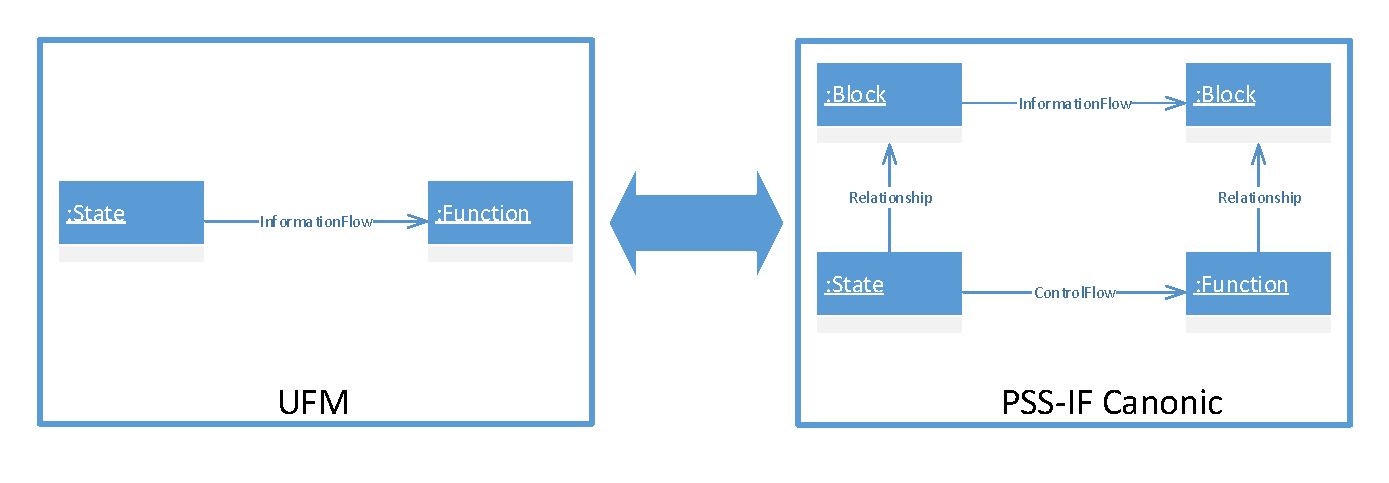
\includegraphics[width=\textwidth]{figures/transformation.pdf}
\caption{Example Transformation}
\label{fig:transformation}
\end{figure}

This viewpoint results in the transformation depicted in \figref{fig:transformation}. Since the behaviour of the \texttt{Viewpoint} is independent of the particular kind of transformation used, the definition of a \texttt{Viewpoint} is reduced to the definition of all necessary transformations and their combination in the appropriate order. The current set of available transformation covers all the ones described in \chapref{chap:approach}.

\subsection{Generic Graph}

A simple component used for intermediate steps in the transformation process is the generic graph component of the PSS-IF \gls{poc}. This component is a simple undirected graph consisting of nodes and edges, which can have string-named attributes with string values, as well as the name of their assumed type. A UML Class Diagram describing the generic graph is depicted in \figref{fig:genericgraph}. In this sense, the graph is an untyped and unstructured equivalent of a PSS-IF Model.

\begin{figure}[h]
\centering
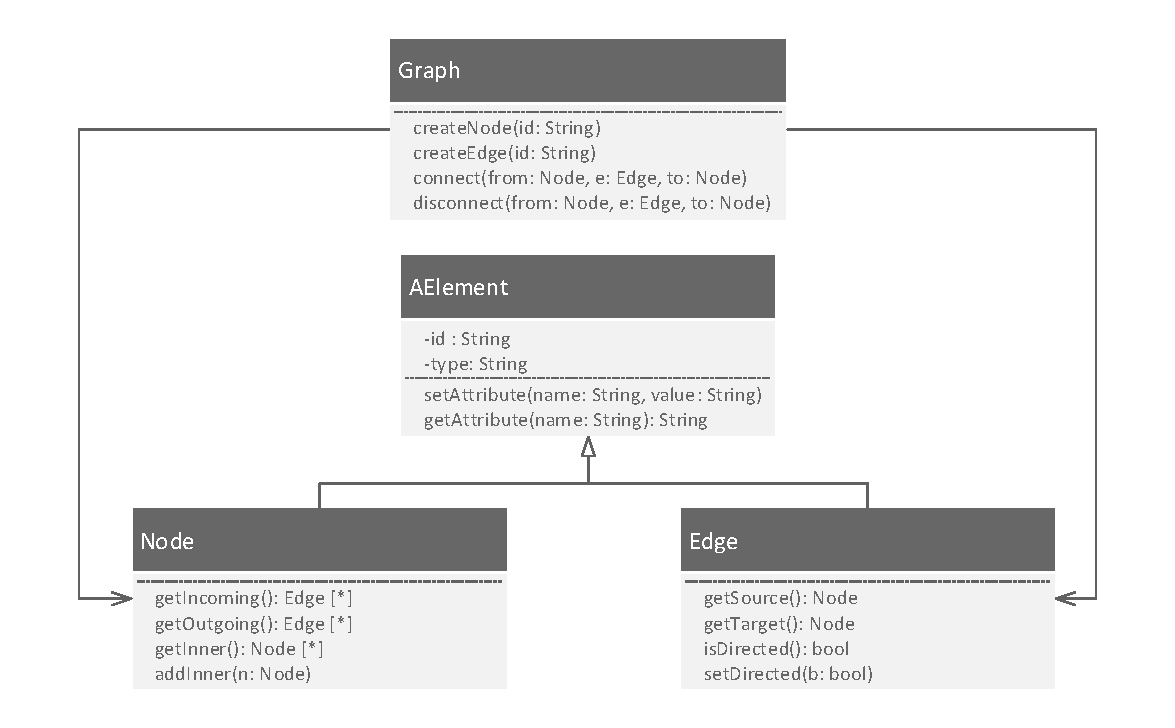
\includegraphics[scale=0.75]{figures/graph.pdf}
\caption{UML Class Diagram of the Generic Graph}
\label{fig:genericgraph}
\end{figure}

In the transformation process, the generic graph is used as an intermediate format, separating the concrete syntax and the abstract syntax of each supported language. The concrete syntax is defined by the file provided by the user and is handled by an \texttt{IoMapper} (see \secref{sec:impl:comp:io}), while the abstract syntax is defined by the \texttt{Viewpoint} and is processed by a \texttt{ModelMapper} (see \secref{sec:impl:comp:model}). The details of the process are provided in \secref{sec:impl:process}.

\subsection{I/O Mappers}
\label{sec:impl:comp:io}

The I/O Mapper component is responsible for the serialization and de-serialization of a generic graph to and from a stream. In this sense, the component has the task to abstract over the concrete syntax used for the representation of the user's data in any particular language. The API of the component is the \texttt{IoMapper} interface, which has the following signature:

\begin{itemize}
\item \texttt{Graph read(InputStream in);}
\item \texttt{void write(Graph graph, OutputStream out);}
\end{itemize}

The same \texttt{IoMapper} may be used for more than one language. For example, the \texttt{VsdxIoMapper} could be used for both, EPC and BPMN.

\subsection{Model Mappers}
\label{sec:impl:comp:model}

The Model Mapper component is responsible for the translation between generic graphs and PSS-IF Models under the provision of a corresponding PSS-IF \texttt{Viewpoint} (Metamodel). In this sense, it handles the translation between the abstract syntax of the external representation and the abstract syntax of the language's viewpoint in PSS-IF. The component is realized through the \texttt{ModelMapper} interface, which has the following signature:

\begin{itemize}
\item \texttt{Model read(Metamodel metamodel, Graph graph);}
\item \texttt{Graph write(Metamodel metamodel, Model model);}
\end{itemize}

In the simplest case, a particular model mapper would simply use the provided viewpoint to directly transfer information between a Model and a graph, processing all nodes, edges and attributes. In more complex cases, pre- or post-processing of the graph may be necessary, to ''normalize'' it into a structure compatible with the viewpoint defined for the particular language (and, hence, with the provided Model). This may, for example, be the case, if the external representation requires the nodes of a graph to be ordered in accordance with a certain rule, or if there are implicit existential dependencies between nodes, implied by the nature of the \texttt{Viewpoint} or a specific \texttt{Transformation}.

In general, it is assumed that one \texttt{ModelMapper} implementation is necessary for each \gls{dsl} to be supported. Theoretically, if the same language is to be imported from or exported to more than one format, and the generic graph is sufficient to express the abstract syntax of both external formats, the same \texttt{ModelMapper} and \texttt{Viewpoint} can be used with different \texttt{IoMapper} implementations, to obtain different serializations of the same data.

\subsection{Microsoft Visio VSDX I/O}

For the serialization and de-serialization of Microsoft Visio 2013 VSDX files needed to support EPC and BPMN, a special component was developed in a dedicated maven module. The component defines an API for the manipulation of VSDX files, operating with the following abstractions:

\begin{itemize}
\item \texttt{VsdxDocument} An object-oriented representation of an entire VSDX document.
\item \texttt{VsdxPage} A page within a VSDX document.
\item \texttt{VsdxMaster} A master shape defined within a VSDX document.
\item \texttt{VsdxShape} A shape, contained either in a page, or in another shape.
\item \texttt{VsdxConnector} A connector shape, i.e. a shape which connects two other shapes.
\end{itemize}

The inter-relation of the different concepts of the VSDX API is depicted in \figref{fig:vsdxapi}.

\begin{figure}[h]
\centering
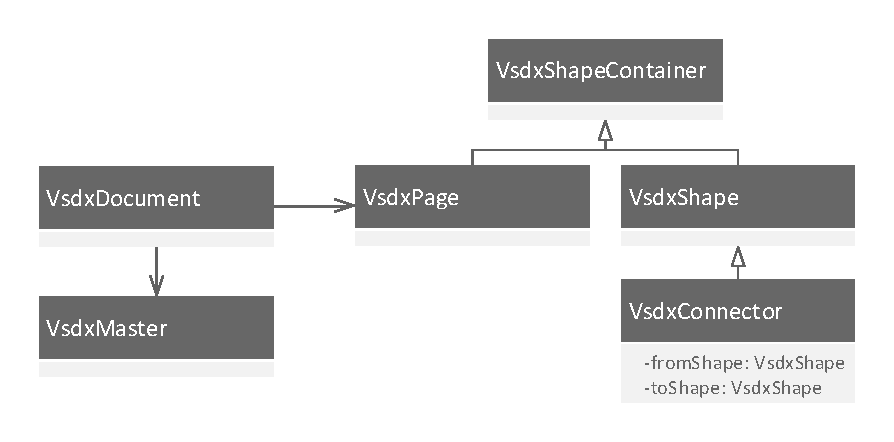
\includegraphics[scale=0.75]{figures/visio.pdf}
\caption{API of the VSDX Component}
\label{fig:vsdxapi}
\end{figure}

It should be noted that the current VSDX component does not provide any mechanisms for layouting, colouring, or other finer operations on a Visio file. This is because the component is aimed explicitly at the extraction and generation of data. The layout of Visio files exported from PSS-IF can be fixed through the usage of algorithms which are built-in in Microsoft Visio. If special decoration of shapes is required, the users can provide their own template files with correspondingly modified master shapes. These template files can then be used in combination with the VSDX component to produce appropriately formatted Visio files. Finally, the API can be extended in future works, to support finer layouting and formatting operations.

\section{Mapping Process}
\label{sec:impl:process}

After, in the previous section, the different components of the PSS-IF \gls{poc} were presented, this section focuses on how the components are tied together and describes the mapping (import and export) process in detail. Here, the term mapping is used, as it covers the processes in both directions and the PSS-IF \gls{poc} implementation handles both cases in the same fashion.

\paragraph{API} The mapping processes are triggered over the corresponding API, represented by the \texttt{Mapper} interface, which has the following signature:

\begin{itemize}
\item \texttt{Model read(Metamodel metamodel, InputStream inputStream);}
\item \texttt{void write(Metamodel metamodel, Model model,}\\ \texttt{OutputStream outputStream);}
\end{itemize}

\paragraph{Implementation} While each specific language, for each file format, requires its own \texttt{Mapper} implementation, the internal procedure for all languages and file formats is the same and is described by the \texttt{AbstractMapper} class, which is the super-class of all \texttt{Mapper} implementations. The \texttt{AbstractMapper} defines the methods of the \texttt{Mapper} API as follows:

\begin{verbatim}
public abstract class AbstractMapper implements Mapper {

 @Override
  public final Model read(Metamodel mm, InputStream in) {
    Graph graph = getIoMapper().read(in);
    Metamodel view = getView(mm);
    ModelMapper modelMapper = getModelMapper();
    return modelMapper.read(view, graph);
  }

  @Override
  public final void write(Metamodel mm, Model m, 
      OutputStream out) {
    Metamodel view = getView(mm);
    ModelMapper modelMapper = getModelMapper();
    Graph graph = modelMapper.write(view, m);
    getIoMapper().write(graph, out);
  }

  protected abstract Metamodel getView(Metamodel metamodel);

  protected abstract ModelMapper getModelMapper();

  protected abstract IoMapper getIoMapper();
 }
\end{verbatim}

As the code above demonstrates, a PSS-IF \texttt{Model} instance is obtained from an external representation by transcoding the external representation into a generic graph, obtaining the \texttt{Viewpoint} of the current language and finally mapping the generic graph to a model in accordance with the viewpoint.

Symmetrically, a file is generated from a PSS-IF \texttt{Model} by first obtaining the \texttt{View\-point} for the current language and using it to translate the model into a generic graph, and then serializing the graph to a stream through the corresponding \texttt{IoMapper}.

\paragraph{Process}

Recall the 6-step process described in \secref{sec:approach:pssif:nutshell}, which describes the transformation process on the conceptual level. In the PSS-IF \gls{poc}, the transformation process is implemented through the consequent invocation of two mappers. The first one is the mapper which de-serializes the source data and transforms it into a Model conforming to the PSS-IF Canonic Metamodel. The second mapper is the one for the target format and is used to write the obtained model into an external representation. For an exemplary source language A and target language B, the Java code describing the transformation process is the following:

\begin{verbatim}
public void transform(Mapper aMapper, Mapper bMapper,
  InputStream inputStream, OutputStream outputStream) {
  
  Metamodel metamodel = PSSIFCanonicMetamodelCreator.create();
  Model model = aMapper.read(metamodel, inputStream);
  bMapper.write(metamodel, model, outputStream);
}
\end{verbatim}

\begin{figure}[h]
\centering
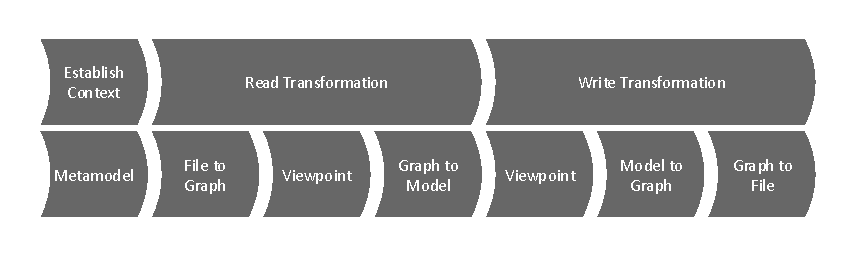
\includegraphics[width=0.8\textwidth]{figures/process.pdf}
\caption{The Transformation Process of the PSS-IF \gls{poc}}
\label{fig:transformationprocess}
\end{figure}

In \figref{fig:transformationprocess}, the transformation process is depicted in two levels of abstraction. The first level addresses the separation into two distinct read and write steps, while the second level demonstrates how both the read and write processes are accomplished by the respective language mappers.
